\clearpage
\section{Stepper motor}
Stepper motors are electrical motors that can be precisely controlled. They divide a full rotation into a discrete amount of steps, each equally big.

Stepper motors are usually used with a specific circuit to control them, which is called a stepper-motor controller. Stepper-motor controllers allow for micro-stepping, which further divides a step into smaller pieces. We used 8 micro-steps per step.

\begin{figure}[H]
	\centering
	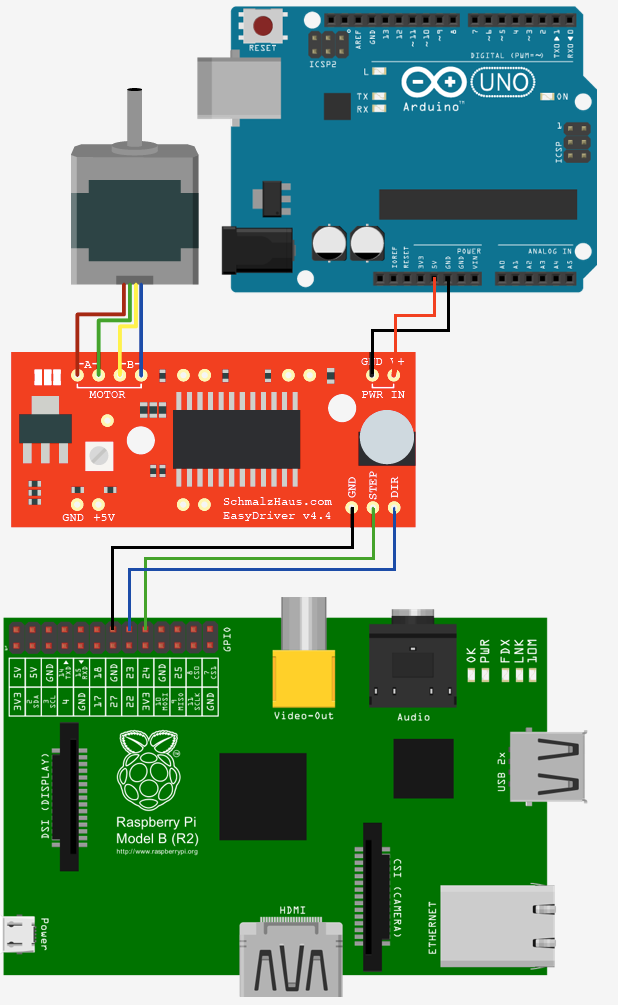
\includegraphics[scale=.5]{images/steppermotor.png}
	\caption{Connection chart for the stepper-motor}
	\label{fig:steppermotor}
\end{figure}

This diagram depicts how we connected the Pi to the stepper-motor, using a motor controller and an arduino in the process.
The only use of the arduino in this picture is to serve as a 5V source, as we were already using the Pi to power the laser.

The stepper motor we used in our project is a NEMA-17 Bipolar Stepper Motor~\cite{steppermotor}.
The stepper motor controller we used is an EasyDriver~\cite{steppercontroller}.

\lstinputlisting[firstline=1, lastline=20, title=Arduino\_Code, language=C++, label=arduinocode1]{../code/arduino_code.cpp}

Since the stepper motor we use divides a full cycle into 200 steps, this means that the resolution is 1.8$\degree$ per step. With this, the we can calculate the minimum distance we can resolve.

$\frac{x}{sin(1.8deg)} = \frac{1m}{sin(89.1deg)}$ \\
$x = \frac{sin(1.8deg)}{sin(89.1deg)}m$ \\
$x = 3.14cm$ \\

At a distance of 1m, 1.8$\degree$ can resolve a distance of ~3.1cm, and this increases linearly with a larger distance (Code reference~\ref{arduinocode1}).
